\section{Application}
This section demonstrates the application of the gradient boosting machine to function approximation. Specifically, we employ a synthetic dataset simulated from the sinc function\footnote{See https://www.rdocumentation.org/packages/qrnn/versions/1.1.3/topics/sinc}. The simulated sinc dataset, a common benchmark for assessing regression models, comprises 200 data points evenly distributed between -10 and 10. These points are derived from a noisy sinc function, defined as sinc(x) = sin(x)/x, with Gaussian noise of mean 0 and standard deviation 0.1 added to the true function. The objective of the regression task is to learn the underlying function from this noisy data. The simulated sinc dataset serves as an effective tool for evaluating the precision and generalizability of various regression models, including gradient boosting models.

\subsection{Function Approximation}
In this subsection, we apply the revised gradient boosting machine to a simulated dataset. The sinc function dataset was divided into training and testing sets, with the model trained on the former and evaluated using the latter.

Figure \ref{fig:contrast} illustrates the results. We initially compared the performance of the Gradient Boosted Decision Trees (GBDT) on the testing set. The model leveraging the revised gradient approach (denoted by the blue curve on the learning curve) demonstrated a faster initial descent rate and lower testing error. For kernel-based learners (Gaussian kernels used for illustrative purposes), the gradient-enhanced model significantly reduced testing errors during the early iterations, but it gradually converged post-200 iterations. When we combined Reproducing Kernel Hilbert Space (RKHS) with decision trees, the testing error didn't consistently improve, which is understandable given our goal of fitting a smooth function, where the RKHS-based gradient boosting model has a natural advantage. Consequently, the combined model didn't outperform the individual models, as expected.

Figures 3 and 4 portray the model fitting process. It is evident that the revised gradient boosting algorithm (represented by the blue curve) better approximates the sample points and achieves favorable results with few iterations while maintaining other parameters constant. It's noteworthy that due to the small sample size, the model quickly begins to overfit. Moreover, when the base learner is an RKHS, the improved model can also accelerate the model's convergence speed.
\begin{figure}[htb]
	\centering
	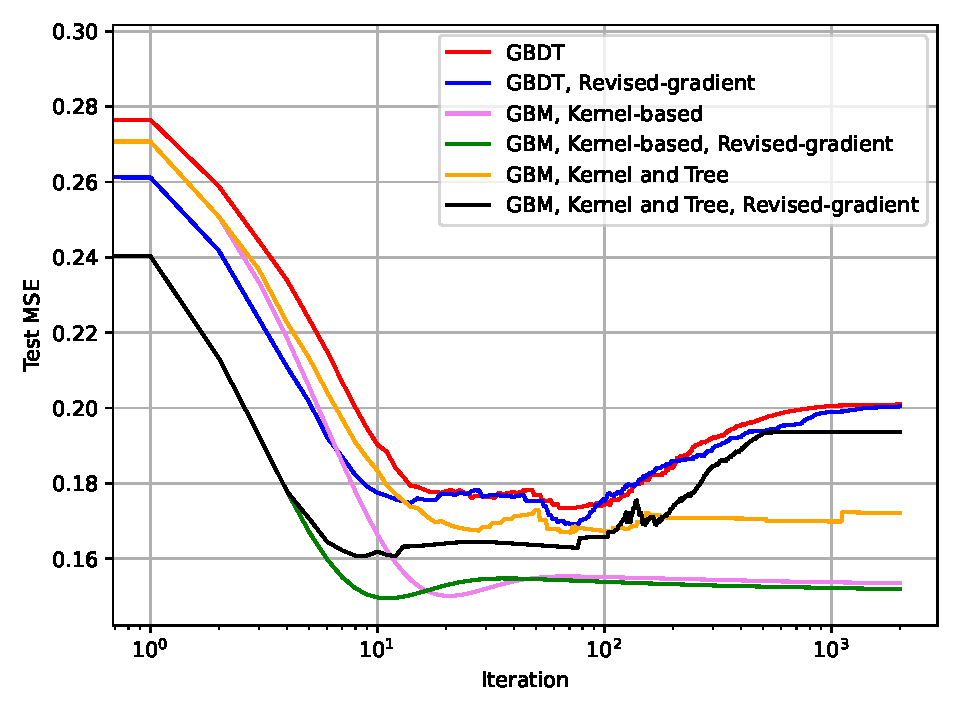
\includegraphics[height=10cm]{figure/test.pdf}
	\caption{Test MSE versus the number of iteration for comparing GBM with/without revised gradient.}
	\label{fig:contrast}
\end{figure}

\begin{figure}[htb]
	\centering
	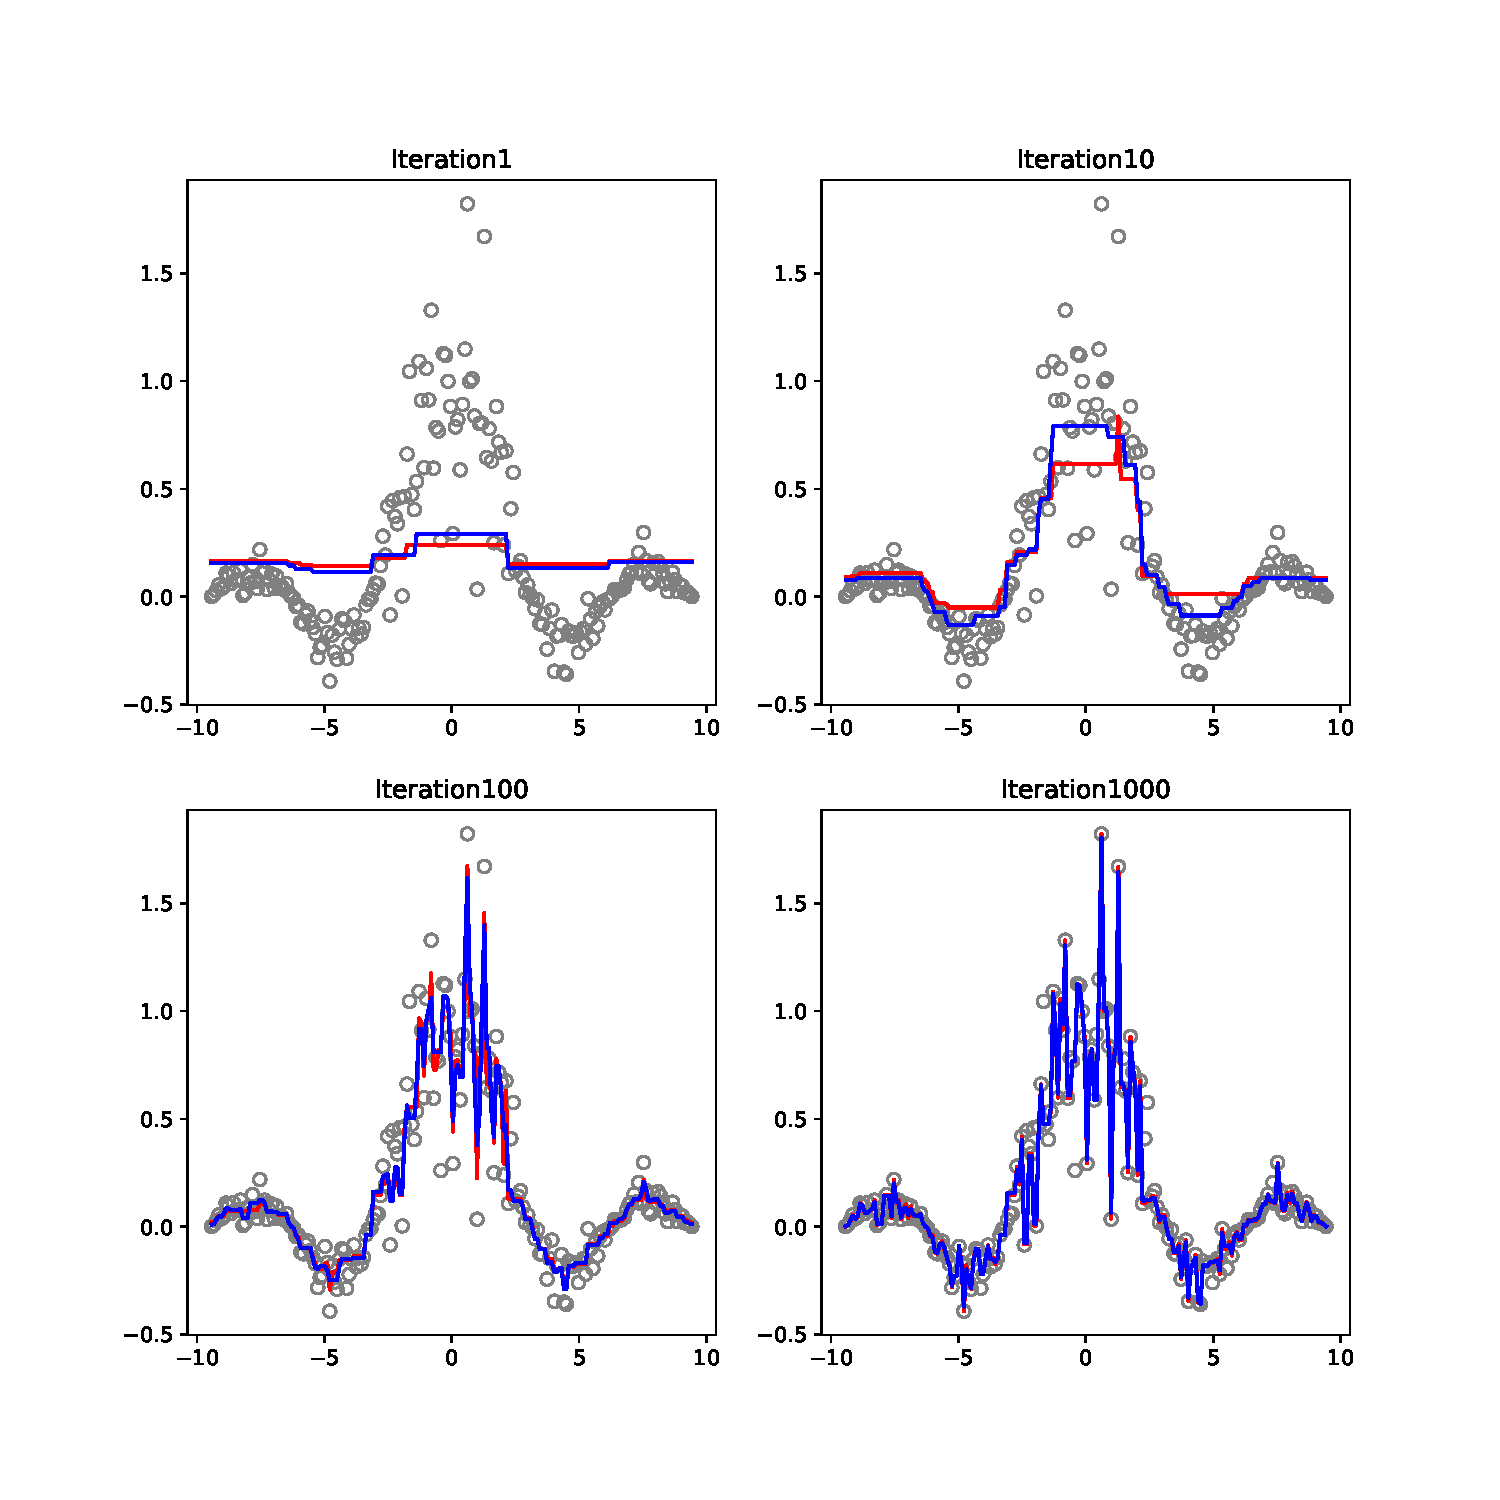
\includegraphics[height=15cm]{figure/train_process_1.pdf}
	\caption{Training process of GBDT.}
\end{figure}

\begin{figure}[htb]
	\centering
	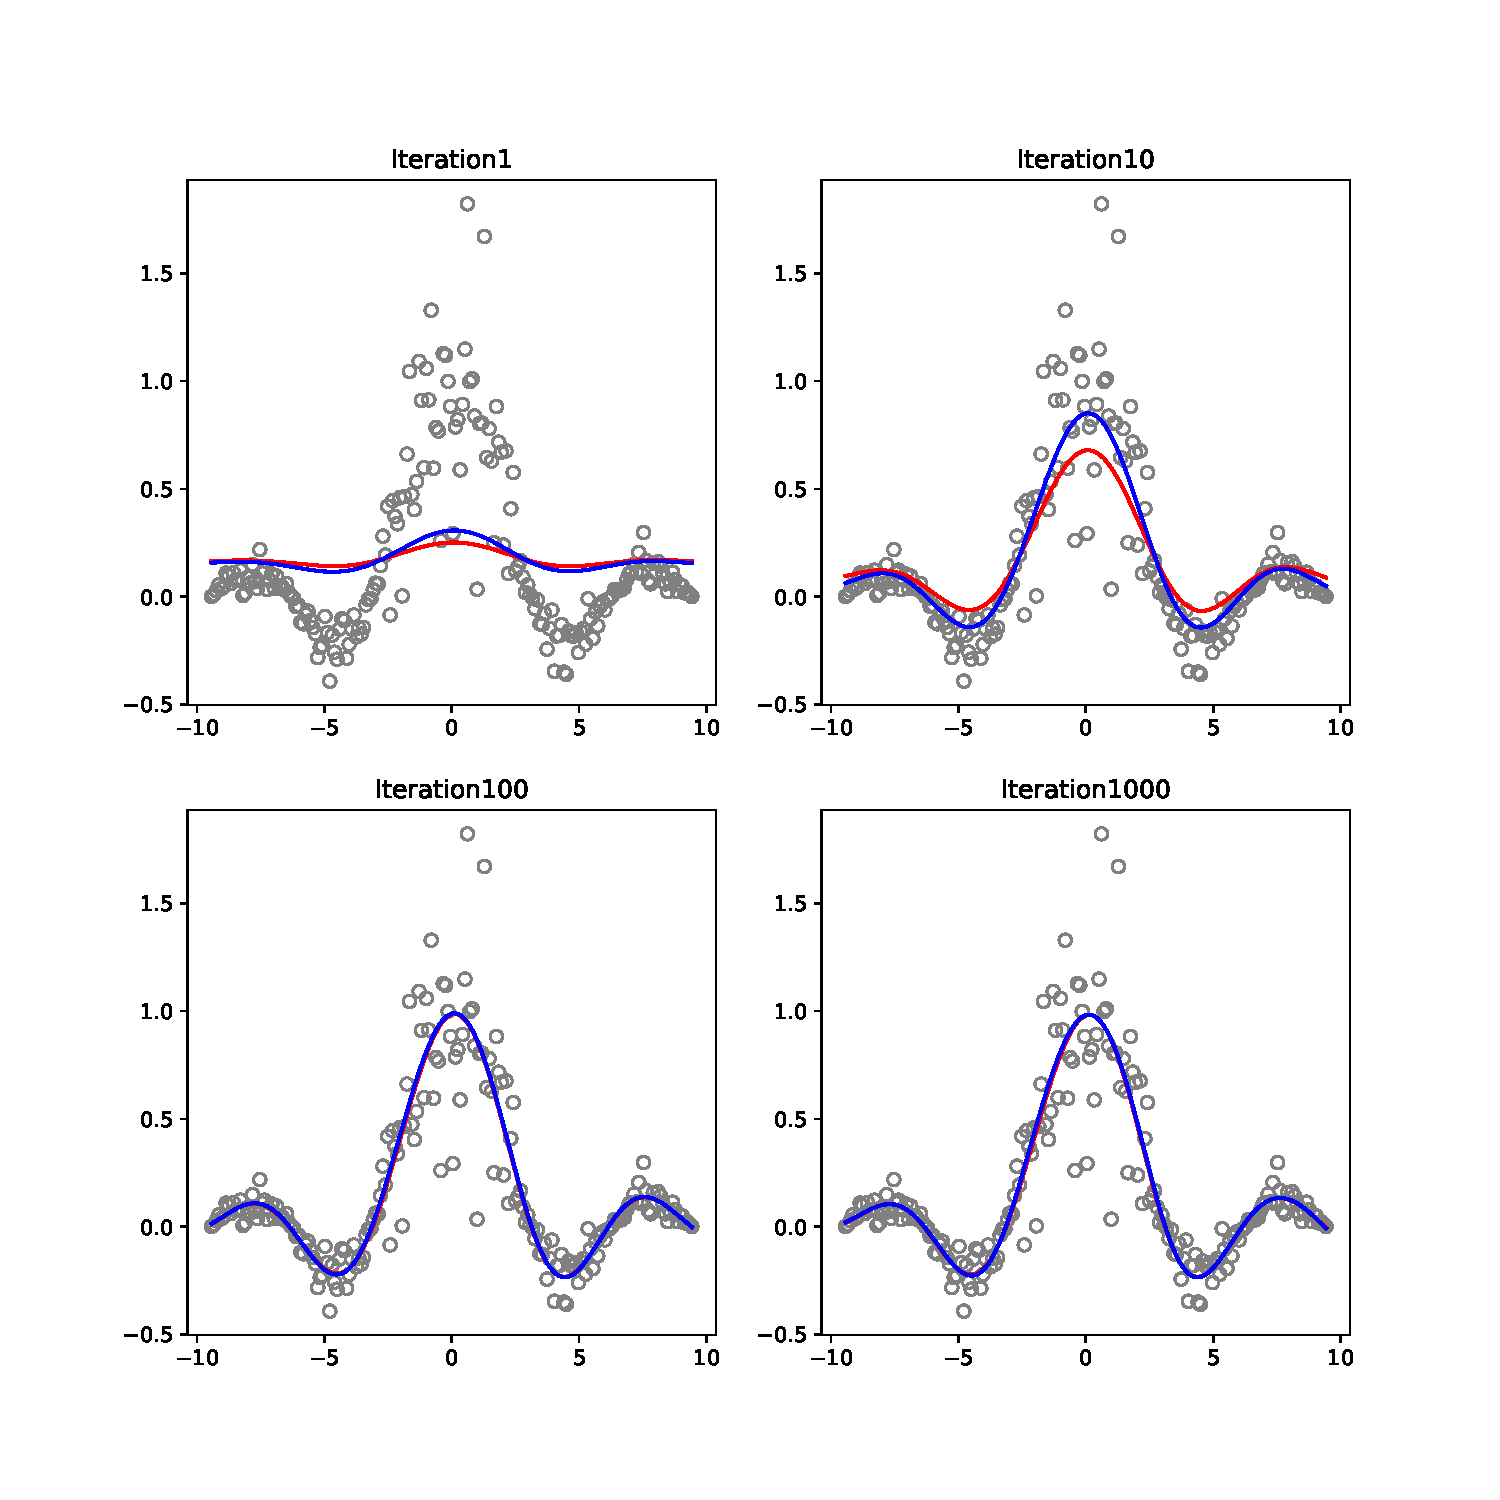
\includegraphics[height=15cm]{figure/train_process_k.pdf}
	\caption{Training process of GBM based on RKHS.}
\end{figure}





%\subsection{Event-Driven Backtesting}
%
%In this subsection, we will introduce some concepts in quantitative finance. 
%%For those who wish to learn more, we recommend visiting https://www.quantstart.com/. Established in 2012, QuantStart is an online resource for mathematical finance articles and tutorials on derivatives pricing, created to assist aspiring quants in obtaining a role in quantitative finance.
%
%There are two main frameworks in quantitative finance: vectorized backtester and event-driven backtester. While both are popular, event-driven systems provide several advantages over a vectorized approach:
%\begin{itemize}
%	
%\item \textbf{Code Reuse}: An event-driven backtester can be used for historical backtesting and live trading with minimal component switching. In contrast, vectorized backtesters require all data to be available simultaneously for statistical analysis.
%\item \textbf{Lookahead Bias}: Event-driven backtesters eliminate lookahead bias by treating market data receipt as an "event" that must be acted upon. As a result, it is possible to "drip feed" an event-driven backtester with market data, replicating how an order management and portfolio system would behave.
%\item \textbf{Realism}: Event-driven backtesters allow for significant customization over how orders are executed and transaction costs are incurred. Essential market and limit orders, as well as market-on-open (MOO) and market-on-close (MOC) orders, can be easily handled by constructing a custom exchange handler.
%\end{itemize}
%Although event-driven systems have numerous benefits, they have two significant drawbacks compared to simpler vectorized systems. Firstly, they are more complicated to implement and test due to having more "moving parts," resulting in a greater risk of introducing bugs. Proper software testing methodology, such as test-driven development, can be employed to mitigate this. Secondly, they are slower to execute than a vectorized system because optimal vectorized operations cannot be used when performing mathematical calculations. 
%
%
%Pytrade is a event-driven trading system developed us. \C{借鉴Uqer,zipline,backtesting,qstrader等多个回测框架,我编写了一个基于事件驱动的量化回测系统,还原了优矿部分 功能,极大程度的避免了量化研究中的前向偏差问题。目前该框架支持策略开发,因子投研,参数优化等功能。在下单方面, 系统充分考虑市场微观结构,支持市价单,限价单,止损单等多种订单。在事件驱动方面,系统利用事件队列的结构,能够处 理新闻数据等另类信息,并同时生成交易信号。}
%
%\begin{figure}[htb]
%\hspace{-2cm}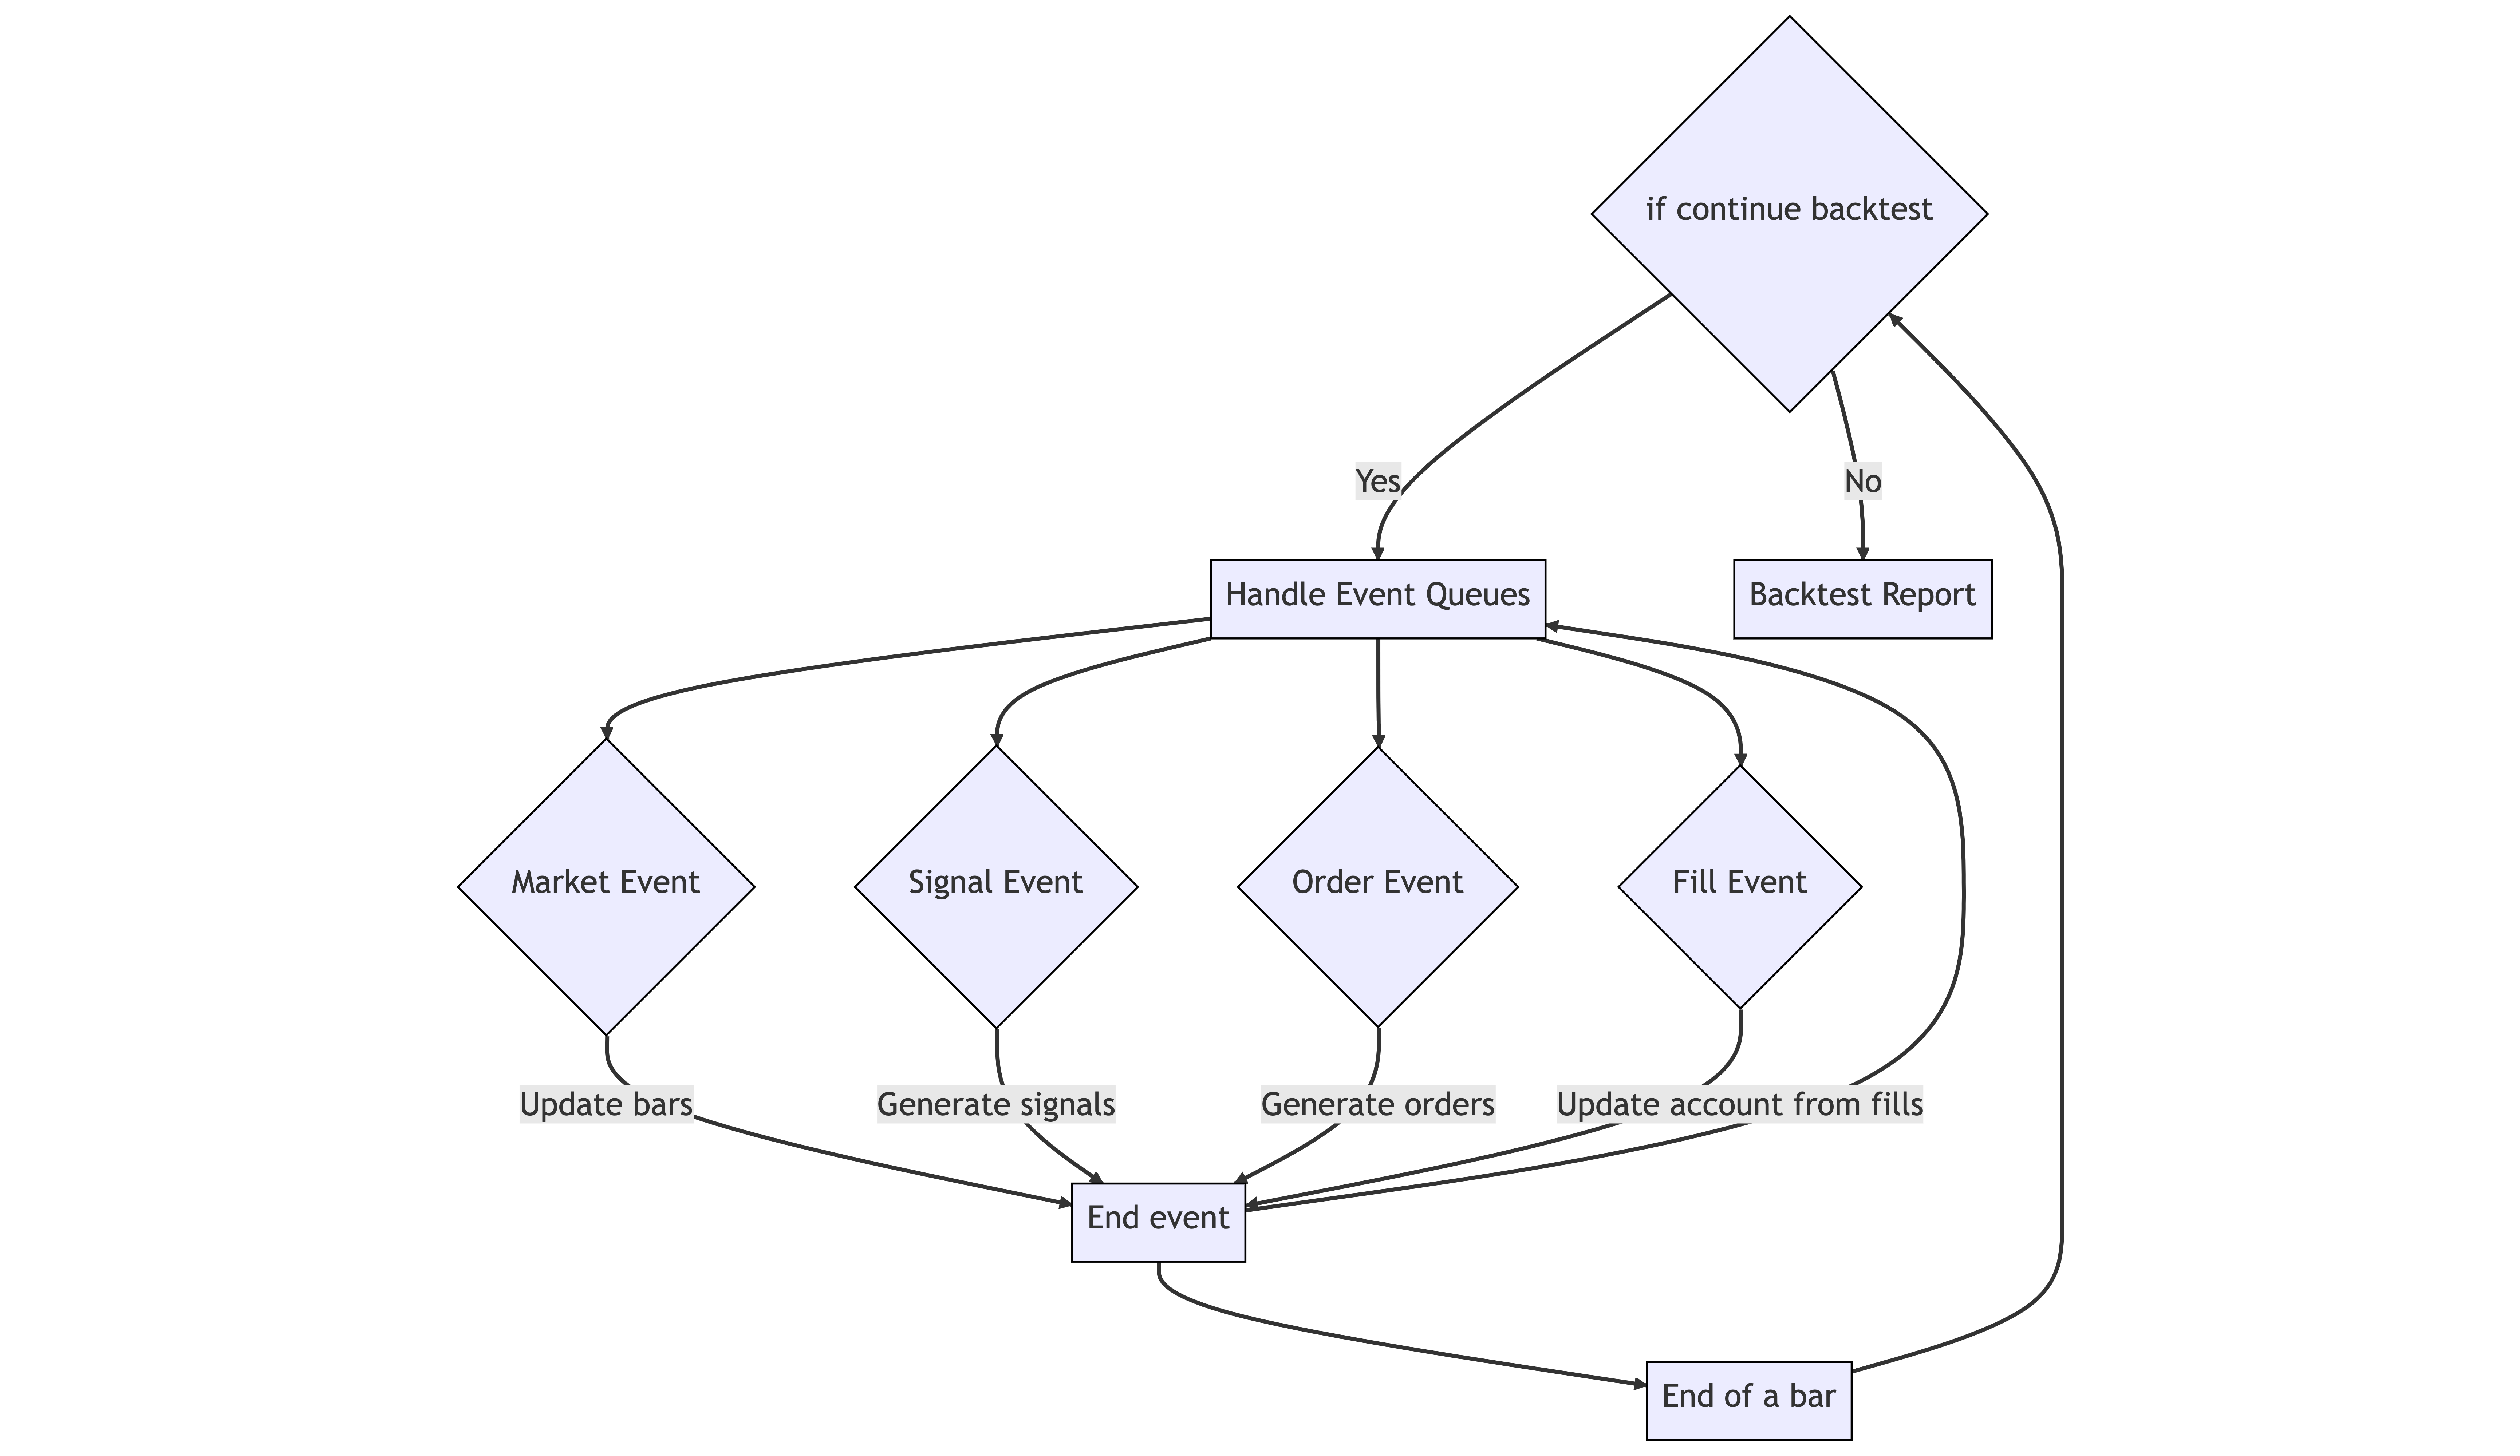
\includegraphics[scale=0.08]{figure/system.png}
%\hspace{-2cm}\caption{Event-Driven Trading System}
%\end{figure}
%




%\subsection{Stock selection based on gradient boosting}
%In stock selection, we need to choose those stocks whose price will rise significantly in the future. 
%\C{在监督学习中, 对数据进行标注至关重要, 我们按照不同的标注方式,将模型分为分类, 回归两类. 在分类问题中, 我们对股票未来一段时间内的收益率进行排序, 前百分之30标记为正, 后百分之30标记为负, }
%\begin{eqnarray*}
%B_t^{+} &=& \left\{ i: CrossQuantile(\frac{C_{t+k}^{(i)} - C_t^{(i)}}{C_t^{(i)}}) > 0.7 \right\} \\
%B_t^{-} &=& \left\{ i: CrossQuantile(\frac{C_{t+k}^{(i)} - C_t^{(i)}}{C_t^{(i)}}) < 0.3 \right\} \\
%\end{eqnarray*}
%$$
%y_t^{(i)} = \chi_{B_t^{+}}(i) -  \chi_{B_t^{-}}(i), \quad i \in B_t^+ \cup B_t^-.
%$$
%\C{而我们认为未来一段时间内收益率分位数为在0.3至0.7之间的数据为噪声, 故将其删除.}
%
%\C{风险度量指标}
%Suppose $r_t$ is the daily(hourly ...) return, then
%\begin{itemize}
%	\item Mean and Volatility 
%	$$ mean(r) = \frac{1}{T}\sum_{t=1}^{T} r_t, \quad $$
%	\item Maxdrawdown:
%	\item Sharpe Ratio:
%	\item Alpha / Excess alpha: 
%	\item Beta:
%	\vspace{1cm}
%	\item Turnover Rate:
%\end{itemize}
%
%\C{而在回归问题中, 我们就有了更多数据标注的方案.}








